
\section{Експериментални резултати}

\subsection{Цел на упражнението}

Целта на това упражнение е да се изследват основните морфологични операции върху бинарни и полутонови изображения. Разглеждат се дилатацията и ерозията като базови операции, тяхното съчетание под формата на отваряне и затваряне, сегментацията на цветни изображения в HSV пространство с помощта на морфологични маски и XOR-базирано извличане на контури, както и bonus задание за разпознаване на цифри чрез template matching. Всяка операция се прилага върху реални изображения и резултатите се анализират качествено.

\section{Резултати и анализ по задания}

\subsection{Задание 1 – Дилатация и влияние на формата на структурния елемент}

\subsubsection{Код}

\begin{lstlisting}[language=Matlab, caption={task1\_dilation.m}]
pkg load image;
clear; close all;

img_dir = '../images/';
out_dir = '../results/';
if ~exist(out_dir, 'dir'); mkdir(out_dir); end

img1 = imread([img_dir 'Dilation.tif']);
img2 = imread([img_dir 'ToiletOpen.tif']);

if size(img1, 3) == 3; img1 = rgb2gray(img1); end
if size(img2, 3) == 3; img2 = rgb2gray(img2); end

% Original SE: 3x3 square (all ones)
SE_orig = strel('square', 3);

% X-type SE: only main and secondary diagonals
SE_x_mat = logical([1 0 1; 0 1 0; 1 0 1]);
SE_x = strel('arbitrary', SE_x_mat);

img1_dil_orig = imdilate(img1, SE_orig);
img1_dil_x    = imdilate(img1, SE_x);
img2_dil_orig = imdilate(img2, SE_orig);
img2_dil_x    = imdilate(img2, SE_x);

imwrite(img1,           [out_dir 'task1_orig_Dilation.png']);
imwrite(img1_dil_orig,  [out_dir 'task1_dil_orig_Dilation.png']);
imwrite(img1_dil_x,     [out_dir 'task1_dil_x_Dilation.png']);
imwrite(img2,           [out_dir 'task1_orig_ToiletOpen.png']);
imwrite(img2_dil_orig,  [out_dir 'task1_dil_orig_ToiletOpen.png']);
imwrite(img2_dil_x,     [out_dir 'task1_dil_x_ToiletOpen.png']);

fig1 = figure('visible', 'off', 'Position', [0 0 1200 400]);
subplot(1,3,1); imshow(img1);          title('Original');
subplot(1,3,2); imshow(img1_dil_orig); title('Dilation - SE 3x3');
subplot(1,3,3); imshow(img1_dil_x);   title('Dilation - SE X');
saveas(fig1, [out_dir 'task1_comparison_Dilation.png']); close(fig1);

fig2 = figure('visible', 'off', 'Position', [0 0 1200 400]);
subplot(1,3,1); imshow(img2);          title('Original');
subplot(1,3,2); imshow(img2_dil_orig); title('Dilation - SE 3x3');
subplot(1,3,3); imshow(img2_dil_x);   title('Dilation - SE X');
saveas(fig2, [out_dir 'task1_comparison_ToiletOpen.png']); close(fig2);

SE_orig_mat = ones(3, 3);
fig3 = figure('visible', 'off', 'Position', [0 0 600 300]);
subplot(1,2,1);
imagesc(SE_orig_mat); colormap(gray); caxis([0 1]);
axis off equal; title('SE original (3x3)');
subplot(1,2,2);
imagesc(double(SE_x_mat)); colormap(gray); caxis([0 1]);
axis off equal; title('SE type X');
saveas(fig3, [out_dir 'task1_se_visualization.png']); close(fig3);
\end{lstlisting}

\subsubsection{Резултати}

Приложена е дилатация върху \textbf{Dilation.tif} и \textbf{ToiletOpen.tif} с два вида структурни елементи: оригинален квадратен SE ($3\times3$, всички единици) и SE тип „X" (единици само по двата диагонала).

\noindent Визуализация на двата структурни елемента:

\begin{figure}[H]
    \centering
    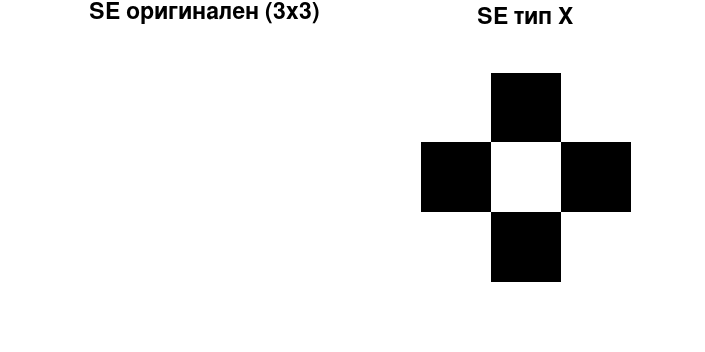
\includegraphics[width=0.5\textwidth]{../results/task1_se_visualization.png}
    \caption{Оригинален SE ($3\times3$) и SE тип „X"}
\end{figure}

\begin{figure}[H]
    \centering
    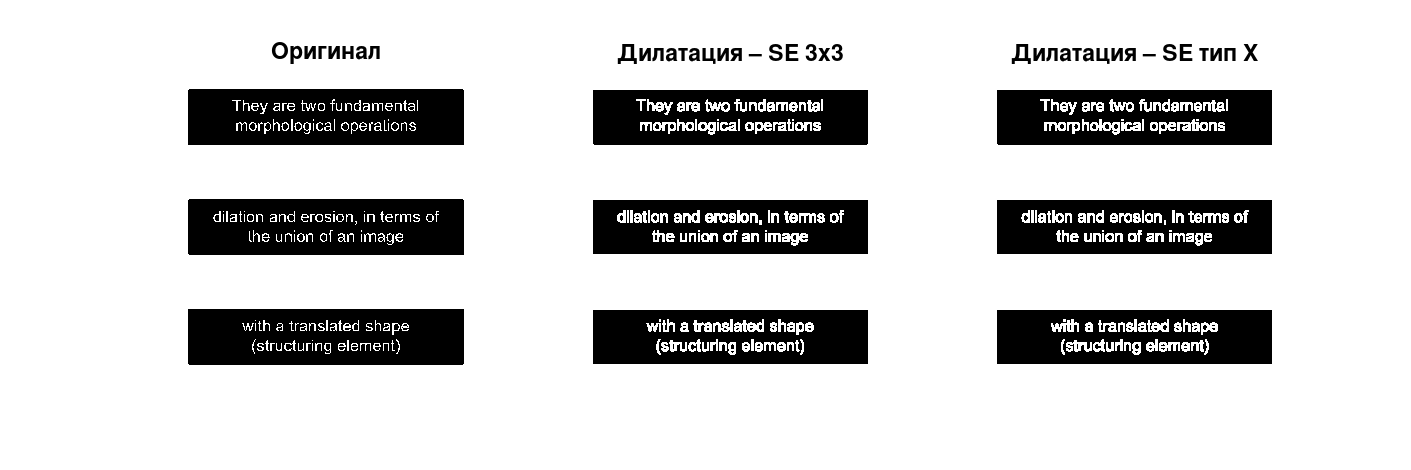
\includegraphics[width=0.95\textwidth]{../results/task1_comparison_Dilation.png}
    \caption{Dilation.tif – оригинал, дилатация с SE $3\times3$, дилатация с SE тип „X"}
\end{figure}

\begin{figure}[H]
    \centering
    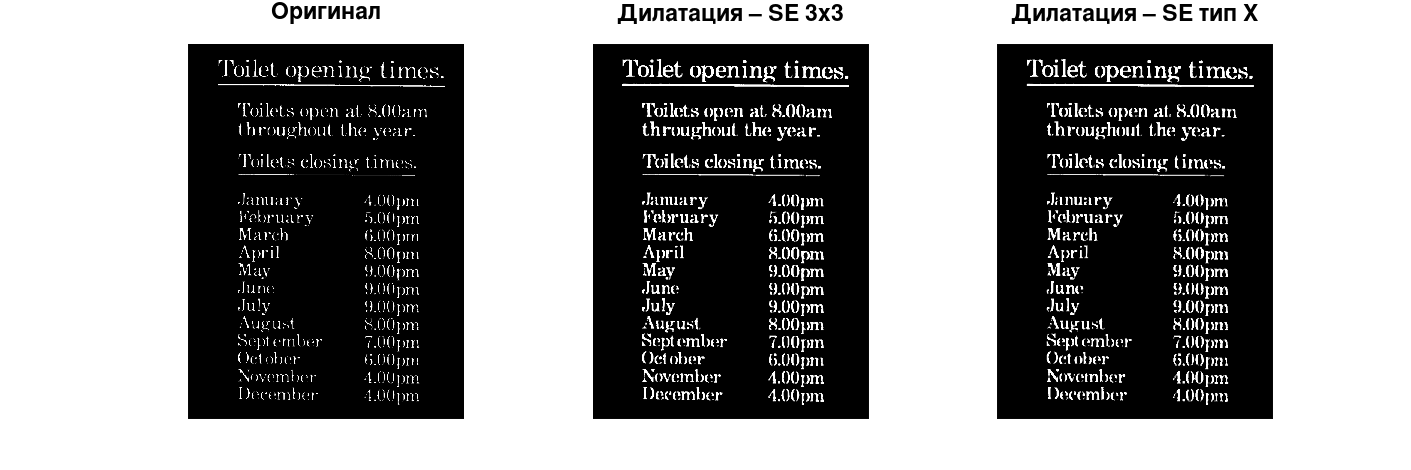
\includegraphics[width=0.95\textwidth]{../results/task1_comparison_ToiletOpen.png}
    \caption{ToiletOpen.tif – оригинал, дилатация с SE $3\times3$, дилатация с SE тип „X"}
\end{figure}

\subsubsection{Анализ}

\textbf{Оригинален SE ($3\times3$, квадратен):} Дилатацията с квадратен SE разширява обектите равномерно във всичките осем посоки – хоризонтално, вертикално и диагонално. Малки отвори и тесни пролуки, ориентирани в произволна посока, се запълват. Контурите на обектите се „нарастват" с по 1 пиксел навсякъде, а близко разположените обекти са склонни да се свържат.

\textbf{SE тип „X":} Дилатацията с X-образен SE разширява обектите само по четирите диагонални посоки. Хоризонталните и вертикалните ръбове се засягат значително по-малко в сравнение с квадратния SE. Диагонално ориентираните линии и структури нарастват по-бързо, докато хоризонтални и вертикални тесни пролуки остават отворени или се запълват по-бавно.

\textbf{Конкретен пример:} При ToiletOpen.tif тесните хоризонтални пролуки между частите на тоалетната седалка се запълват при квадратния SE поради равномерното разширяване. При SE тип „X" тези хоризонтални пролуки остават частично отворени, тъй като разширяването действа предимно диагонално.

\textbf{Качествен ефект:}
\begin{itemize}
    \item \textbf{Тънки линии:} Квадратният SE ги удебелява равномерно; X-типът ги удебелява преди всичко в диагонална посока, придавайки им „назъбен" вид по хоризонтал и вертикал.
    \item \textbf{Малки празнини:} Квадратният SE запълва всички малки дупки; X-типът запълва само диагонално ориентираните.
    \item \textbf{Близко разположени обекти:} Квадратният SE ги свързва при малко разстояние в каквато и да е посока; X-типът свързва само тези, разделени по диагонал.
\end{itemize}

\subsection{Задание 2 – Ерозия със strel: diamond, disk и square}

\subsubsection{Код}

\begin{lstlisting}[language=Matlab, caption={task2\_erosion.m}]
pkg load image;
clear; close all;

img_dir = '../images/';
out_dir = '../results/';
if ~exist(out_dir, 'dir'); mkdir(out_dir); end

img = imread([img_dir 'Erosion.tif']);
if size(img, 3) == 3; img = rgb2gray(img); end

imwrite(img, [out_dir 'task2_original.png']);

params = [2, 4, 6, 8, 10];
types  = {'diamond', 'disk', 'square'};

for t = 1:length(types)
    stype = types{t};

    fig = figure('visible', 'off', 'Position', [0 0 1800 400]);
    subplot(1, 6, 1); imshow(img); title('Original');

    for p = 1:length(params)
        param  = params(p);
        if strcmp(stype, 'disk')
            SE = strel(stype, param, 0);
        else
            SE = strel(stype, param);
        end

        img_er = imerode(img, SE);

        imwrite(img_er, [out_dir 'task2_erode_' stype '_' ...
                         num2str(param) '.png']);

        subplot(1, 6, p+1);
        imshow(img_er);
        title([stype ' ' num2str(param)]);
    end

    saveas(fig, [out_dir 'task2_comparison_' stype '.png']);
    close(fig);
end
\end{lstlisting}

\subsubsection{Резултати}

Ерозията е приложена върху \textbf{Erosion.tif} с три вида структурни елементи (\textit{diamond}, \textit{disk}, \textit{square}) и параметри $D, R, W \in \{2, 4, 6, 8, 10\}$.

\begin{figure}[H]
    \centering
    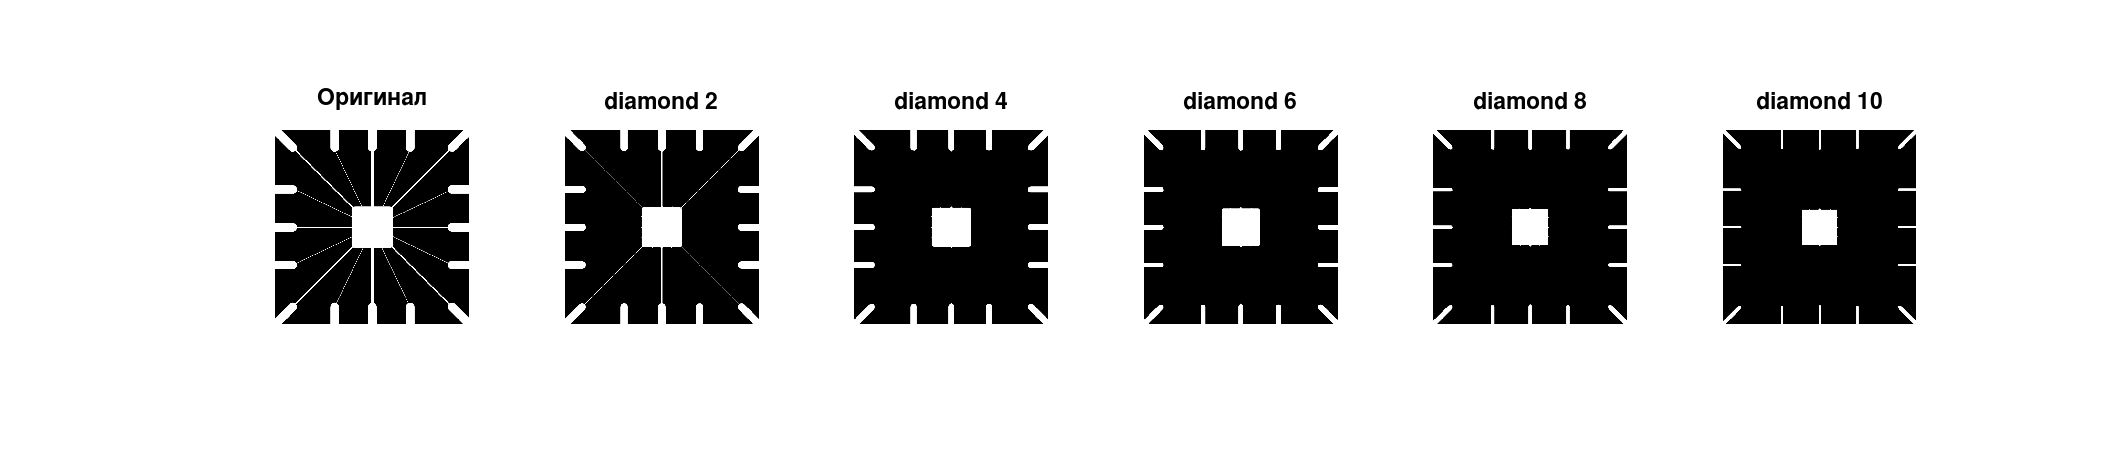
\includegraphics[width=\textwidth]{../results/task2_comparison_diamond.png}
    \caption{Erosion.tif – ерозия с \texttt{diamond} при параметри 2, 4, 6, 8, 10}
\end{figure}

\begin{figure}[H]
    \centering
    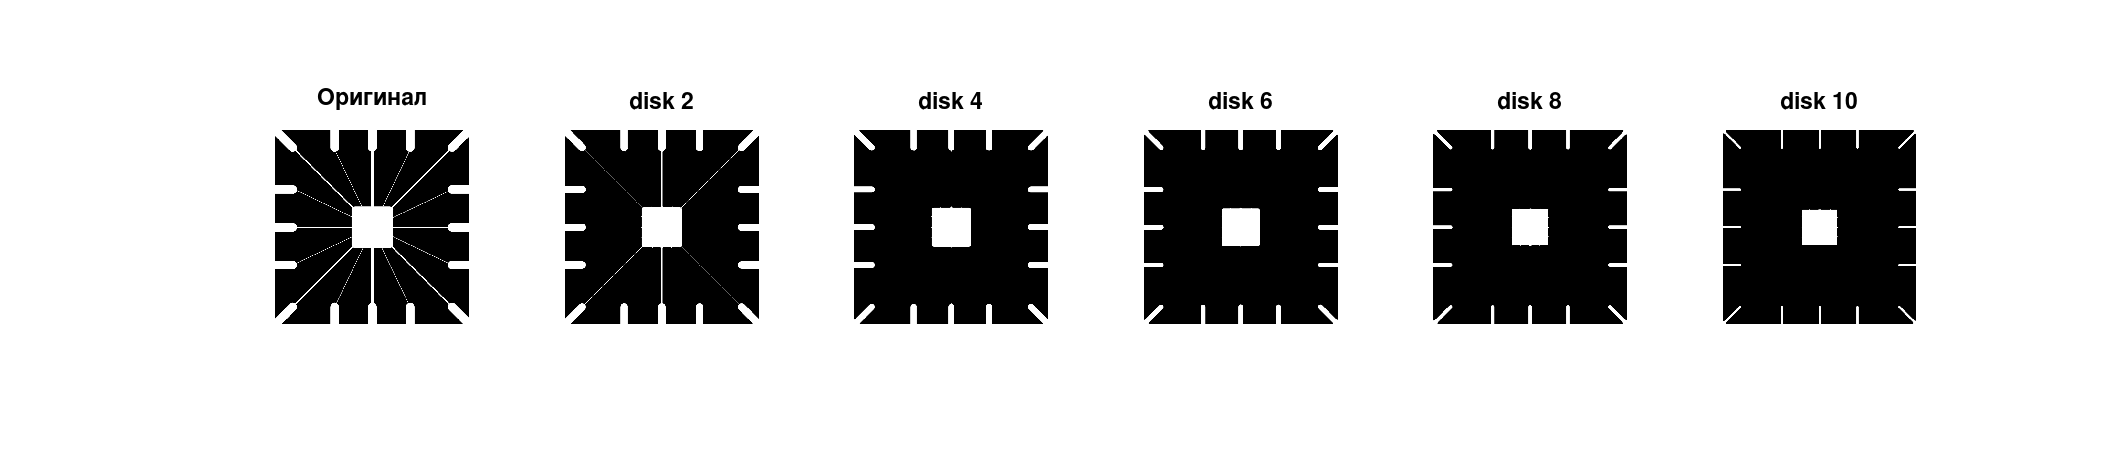
\includegraphics[width=\textwidth]{../results/task2_comparison_disk.png}
    \caption{Erosion.tif – ерозия с \texttt{disk} при параметри 2, 4, 6, 8, 10}
\end{figure}

\begin{figure}[H]
    \centering
    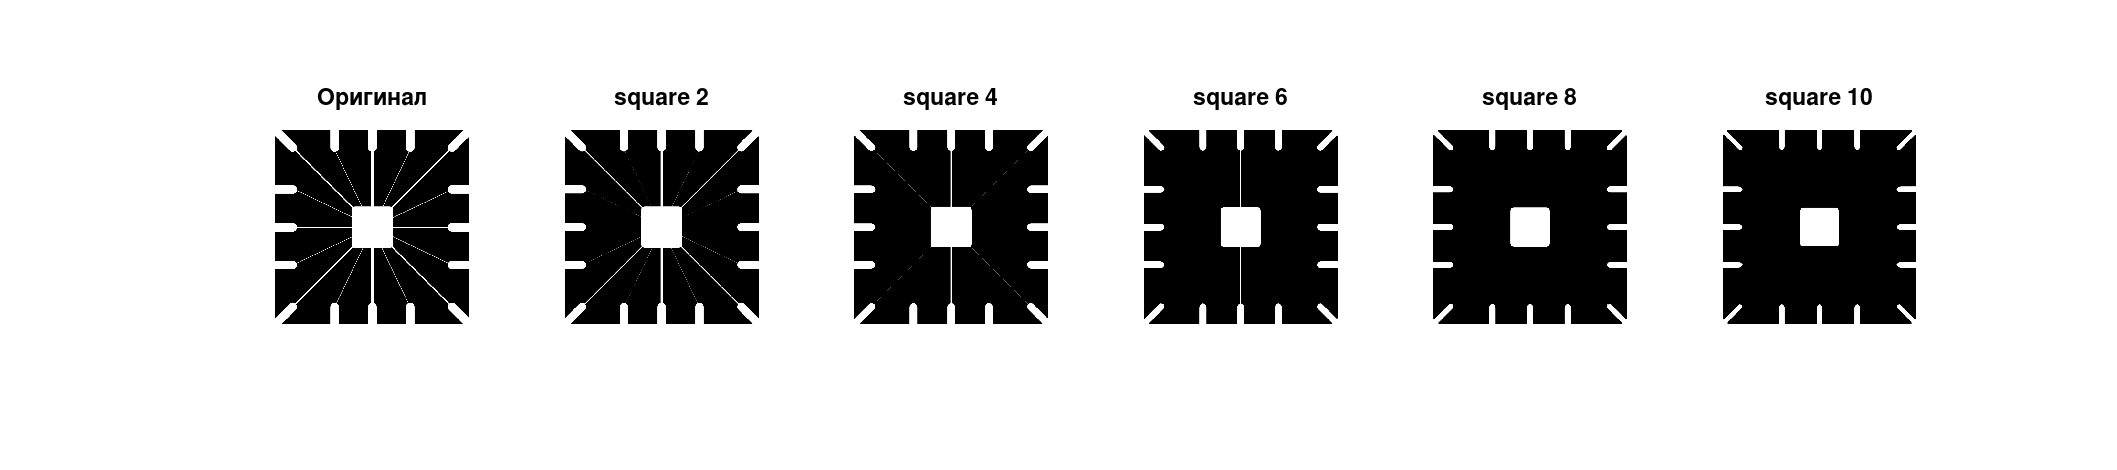
\includegraphics[width=\textwidth]{../results/task2_comparison_square.png}
    \caption{Erosion.tif – ерозия с \texttt{square} при параметри 2, 4, 6, 8, 10}
\end{figure}

\noindent Таблица с качествена оценка на ерозията по тип SE и параметър:

\begin{table}[H]
\centering
\caption{Качествена оценка на ерозията}
\begin{tabular}{llcll}
\toprule
\textbf{SE тип} & \textbf{Параметър} & \textbf{Тънки структури} & \textbf{Контури} & \textbf{Загуба на детайл} \\
\midrule
\multirow{5}{*}{\textbf{diamond}} & 2  & Запазени         & Леко изтъняване   & Минимална \\
                                   & 4  & Частично изчезват & Изтъняване       & Умерена \\
                                   & 6  & Изчезват          & Значителна ерозия & Средна \\
                                   & 8  & Изчезнали         & Силна ерозия      & Висока \\
                                   & 10 & Изчезнали         & Само ядро         & Много висока \\
\midrule
\multirow{5}{*}{\textbf{disk}}    & 2  & Запазени          & Леко изтъняване   & Минимална \\
                                   & 4  & Частично изчезват & Кръгла ерозия     & Умерена \\
                                   & 6  & Изчезват          & Равномерна        & Средна \\
                                   & 8  & Изчезнали         & Силна ерозия      & Висока \\
                                   & 10 & Изчезнали         & Само ядро         & Много висока \\
\midrule
\multirow{5}{*}{\textbf{square}}  & 2  & Леко засегнати    & Правоъгълна       & Лека \\
                                   & 4  & Изчезват          & Силно правоъгълна & Средна \\
                                   & 6  & Изчезнали         & Агресивна         & Висока \\
                                   & 8  & Изчезнали         & Много агресивна   & Много висока \\
                                   & 10 & Изчезнали         & Само ядро         & Максимална \\
\bottomrule
\end{tabular}
\end{table}

\subsubsection{Анализ}

\textbf{Тенденция при нарастване на параметъра:} При всеки тип SE увеличаването на параметъра води до по-агресивна ерозия – обектите се свиват, тънките структури изчезват и в крайна сметка остава само „ядрото" на по-едрите обекти. При малки стойности (2–4) се изтриват само изолираните пиксели и тесните шипове; при средни (4–6) изчезват тънките детайли; при големи (8–10) се запазва само масивното „тяло" на обектите.

\textbf{Сравнение на формите:}
\begin{itemize}
    \item \textbf{diamond:} Ерозира в ромбовидна форма, по-„меко" в ъглите. Диагоналните ъгли на обектите се запазват по-дълго от тези при square. Тънките хоризонтални и вертикални структури изчезват по-бързо от диагоналните.
    \item \textbf{disk:} Дава най-кръгла ерозия. Запазва закръглените контури на обектите без ъглова деформация, тъй като маската е апроксимация на кръг. Закръглените структури в изображението се свиват равномерно и запазват формата си най-добре.
    \item \textbf{square:} Най-агресивният тип – правоъгълната маска премахва повече пиксели за единица параметър в сравнение с другите два. Ъгловите области на обектите се „отрязват" правоъгълно, а тънките детайли изчезват при по-малки стойности на $W$.
\end{itemize}

\textbf{Начало на изчезване на тънки структури:} При \textit{diamond} тънките структури започват да изчезват при $D=4$; при \textit{disk} – при $R=4$; при \textit{square} – вече при $W=2$–$4$ в зависимост от дебелината им. Квадратният SE е най-„агресивен" за изображението, тъй като неговата площ нараства с $W^2$, докато за disk и diamond нарастването е по-бавно.

\textbf{Извод:} Изборът на форма на SE задава „характера" на ерозията. За запазване на закръглени обекти – \textit{disk}; за равномерна ерозия с ромбовиден отпечатък – \textit{diamond}; за максимално „почистване" на фон и тънки детайли – \textit{square}.

\subsection{Задание 3 – HSV сегментация на „язовир" и извличане на контури чрез XOR}

\subsubsection{Код}

\begin{lstlisting}[language=Matlab, caption={task3\_segmentation.m}]
pkg load image;
clear; close all;

img_dir = '../images/';
out_dir = '../results/';
if ~exist(out_dir, 'dir'); mkdir(out_dir); end

images = {'Satellite1', 'Satellite2'};

% HSV thresholds for water/reservoir segmentation (H and S in [0,1])
h_min = [0.50, 0.48];
h_max = [0.72, 0.75];
s_min = [0.15, 0.12];
s_max = [1.00, 1.00];

for k = 1:length(images)
    name    = images{k};
    img_rgb = imread([img_dir name '.tif']);

    img_hsv = rgb2hsv(img_rgb);
    H = img_hsv(:,:,1);
    S = img_hsv(:,:,2);

    mask = (H >= h_min(k)) & (H <= h_max(k)) & ...
           (S >= s_min(k)) & (S <= s_max(k));

    SE = strel('disk', 3, 0);
    mask_morph = imclose(imopen(mask, SE), SE);

    contour_xor = xor(mask, mask_morph);

    imwrite(img_rgb,                      [out_dir 'task3_rgb_'        name '.png']);
    imwrite(im2uint8(H),                  [out_dir 'task3_H_'          name '.png']);
    imwrite(im2uint8(S),                  [out_dir 'task3_S_'          name '.png']);
    imwrite(im2uint8(double(mask)),       [out_dir 'task3_mask_'       name '.png']);
    imwrite(im2uint8(double(mask_morph)), [out_dir 'task3_mask_morph_' name '.png']);
    imwrite(im2uint8(double(contour_xor)),[out_dir 'task3_contour_'    name '.png']);

    fig = figure('visible', 'off', 'Position', [0 0 1800 700]);
    subplot(2,3,1); imshow(img_rgb);    title('RGB original');
    subplot(2,3,2); imshow(H);          title('H channel');
    subplot(2,3,3); imshow(S);          title('S channel');
    subplot(2,3,4); imshow(mask);       title('Mask (threshold)');
    subplot(2,3,5); imshow(mask_morph); title('Mask (morphology)');
    subplot(2,3,6); imshow(contour_xor);title('Contours (XOR)');
    saveas(fig, [out_dir 'task3_comparison_' name '.png']);
    close(fig);
end
\end{lstlisting}

\subsubsection{Резултати}

Приложена е HSV сегментация на водна площ в \textbf{Satellite1.tif} и \textbf{Satellite2.tif}. Каналите H и S са визуализирани, приложен е двоен праг и последваща морфологична обработка с дискообразен SE ($r=3$). Контурите са извлечени чрез XOR между маската преди и след морфология.

\noindent Таблица с използваните прагове:

\begin{table}[H]
\centering
\caption{Прагове по H и S за сегментация на водна площ}
\begin{tabular}{lllll}
\toprule
\textbf{Изображение} & $H_{\min}$ & $H_{\max}$ & $S_{\min}$ & $S_{\max}$ \\
\midrule
Satellite1 & 0.50 & 0.72 & 0.15 & 1.00 \\
Satellite2 & 0.48 & 0.75 & 0.12 & 1.00 \\
\bottomrule
\end{tabular}
\end{table}

\begin{figure}[H]
    \centering
    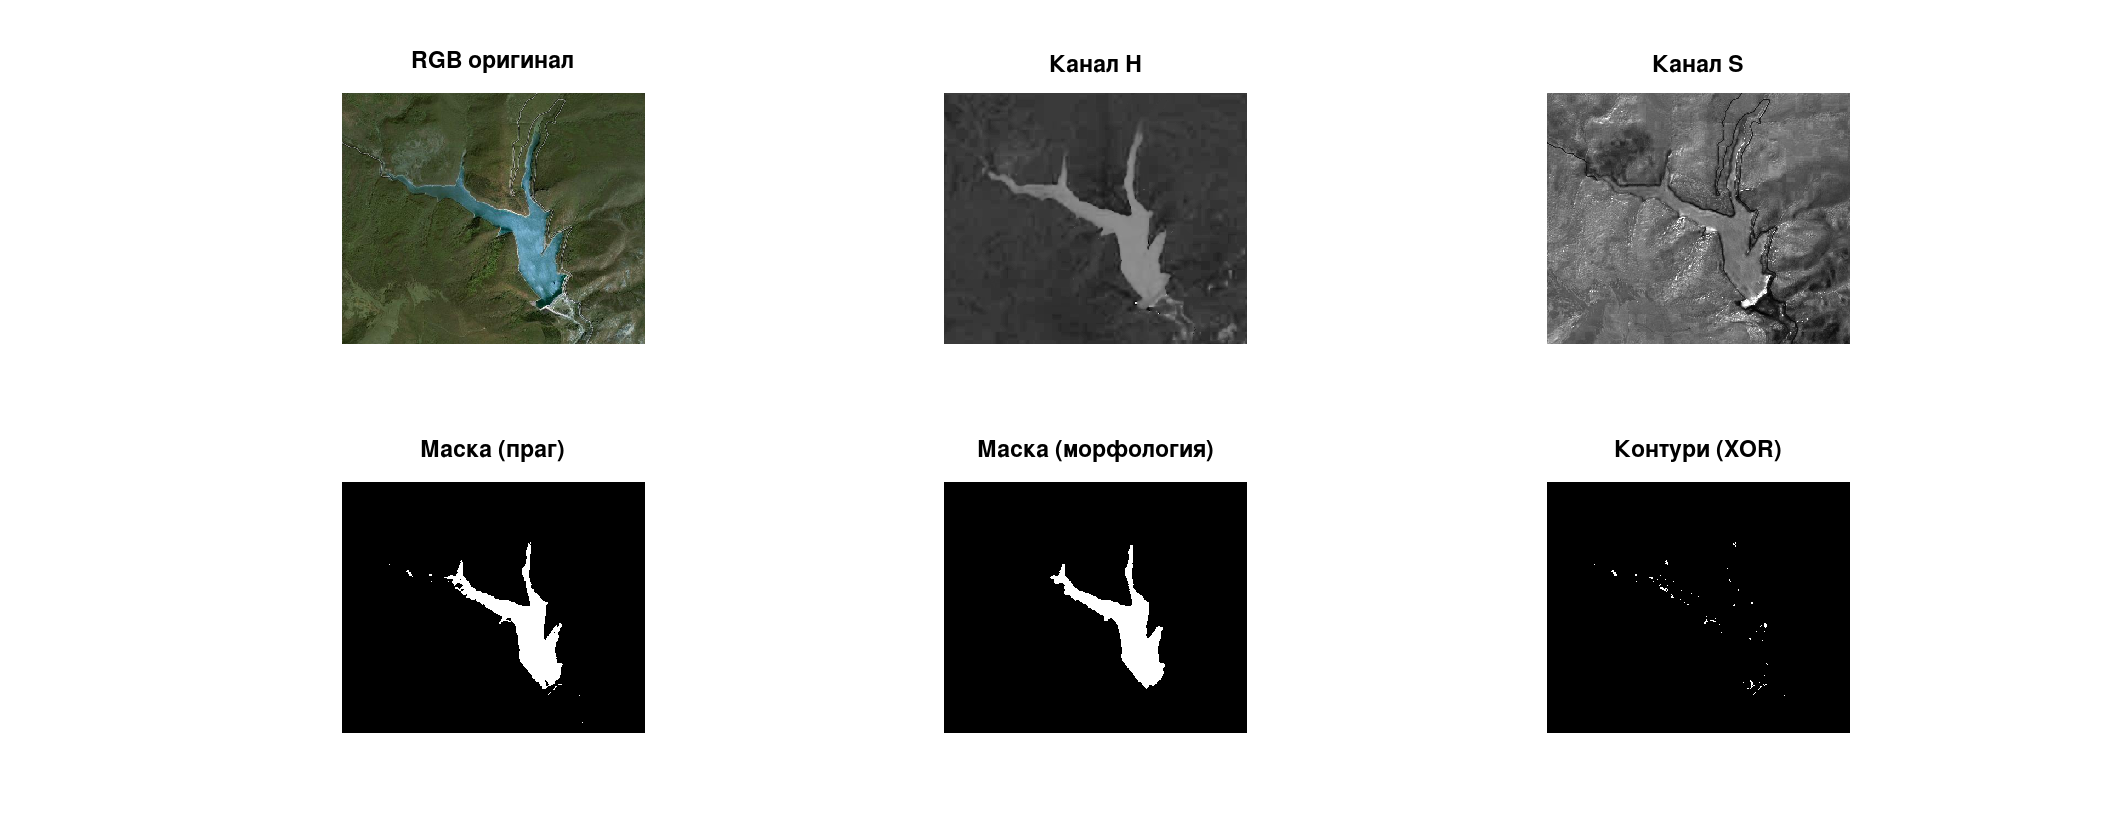
\includegraphics[width=\textwidth]{../results/task3_comparison_Satellite1.png}
    \caption{Satellite1.tif – RGB, H, S, маска (праг), маска (морфология), контури (XOR)}
\end{figure}

\begin{figure}[H]
    \centering
    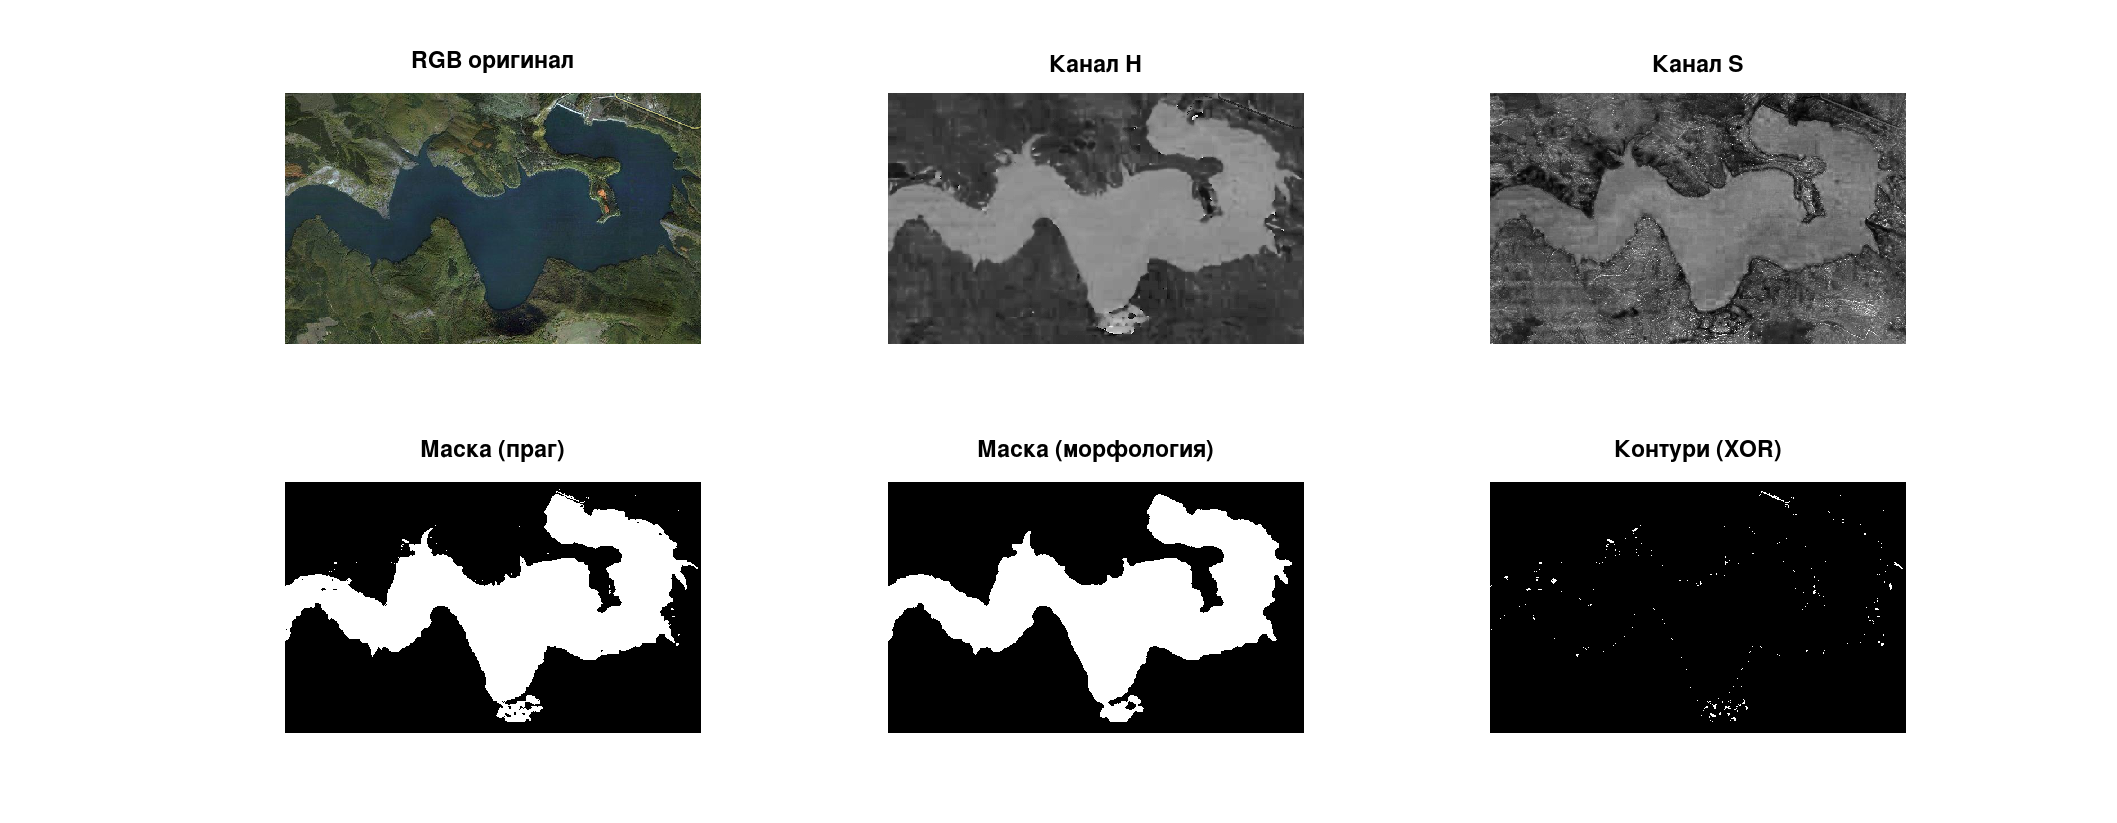
\includegraphics[width=\textwidth]{../results/task3_comparison_Satellite2.png}
    \caption{Satellite2.tif – RGB, H, S, маска (праг), маска (морфология), контури (XOR)}
\end{figure}

\subsubsection{Анализ}

\textbf{Избор на прагове:} Водните площи в сателитни изображения се характеризират с нюанс в синьо-циановия диапазон ($H \approx 0.50$–$0.75$ в нормирана скала $[0,1]$) и умерена наситеност ($S > 0.12$–$0.15$). Горният праг на S е оставен на 1.00, тъй като водата може да бъде силно наситена при ясно небе и дълбок цвят.

\textbf{Satellite1 срещу Satellite2:} Двете изображения изискват леко различни прагове. Satellite2 е с по-ниска наситеност ($S_{\min}=0.12$ вместо 0.15) и по-широк диапазон по H ($H_{\min}=0.48$), което е обяснимо с по-различно осветление или замъгляване на цвета на водата поради по-нисък ъгъл на слънцето, наличие на отражения или различна дълбочина.

\textbf{Роля на морфологията:} Операцията \textit{imopen} (ерозия + дилатация) премахва изолирани единични пиксели и тесни шумови региони, класифицирани фалшиво като вода поради подобен нюанс (напр. сенки, горски покривки). \textit{Imclose} (дилатация + ерозия) след това запълва малки дупки вътре в маската, причинени от блестящи пикове на вълните или пяна. По такъв начин морфологията прави границата на водното тяло по-компактна и гладка.

\textbf{XOR контури:} XOR между маската преди и след морфология дава пикселите, в които двете маски се различават – тоест граничния пояс, добавен или премахнат от морфологията. Тези контури са точни около основната граница на езерото. Паразитни граници се появяват там, където имало малки изолирани сини петна (шум), отстранени при \textit{imopen}.

\subsection{Задание 4 – Отваряне и затваряне за почистване и възстановяване (Fingerprint)}

\subsubsection{Код}

\begin{lstlisting}[language=Matlab, caption={task4\_opening\_closing.m}]
pkg load image;
clear; close all;

img_dir = '../images/';
out_dir = '../results/';
if ~exist(out_dir, 'dir'); mkdir(out_dir); end

img = imread([img_dir 'FingerprintNoise.tif']);
if size(img, 3) == 3; img = rgb2gray(img); end

imwrite(img, [out_dir 'task4_original.png']);

ws = [3, 7];

for i = 1:length(ws)
    W  = ws(i);
    SE = strel('square', W);

    img_open  = imopen(img, SE);
    img_close = imclose(img_open, SE);

    imwrite(img_open,  [out_dir 'task4_open_W'  num2str(W) '.png']);
    imwrite(img_close, [out_dir 'task4_close_W' num2str(W) '.png']);

    fig = figure('visible', 'off', 'Position', [0 0 1200 400]);
    subplot(1,3,1); imshow(img);       title('Original');
    subplot(1,3,2); imshow(img_open);  title(['Opening W=' num2str(W)]);
    subplot(1,3,3); imshow(img_close); title(['Closing W=' num2str(W)]);
    saveas(fig, [out_dir 'task4_comparison_W' num2str(W) '.png']);
    close(fig);
end

SE3 = strel('square', ws(1));  SE7 = strel('square', ws(2));
open3  = imopen(img, SE3);     close3 = imclose(open3, SE3);
open7  = imopen(img, SE7);     close7 = imclose(open7, SE7);

fig_all = figure('visible', 'off', 'Position', [0 0 2000 420]);
subplot(1,5,1); imshow(img);    title('Original');
subplot(1,5,2); imshow(open3);  title(['Opening W=' num2str(ws(1))]);
subplot(1,5,3); imshow(close3); title(['Closing W=' num2str(ws(1))]);
subplot(1,5,4); imshow(open7);  title(['Opening W=' num2str(ws(2))]);
subplot(1,5,5); imshow(close7); title(['Closing W=' num2str(ws(2))]);
saveas(fig_all, [out_dir 'task4_comparison_all.png']);
close(fig_all);
\end{lstlisting}

\subsubsection{Резултати}

Операциите \textit{opening} и \textit{closing} са приложени върху \textbf{FingerprintNoise.tif} с квадратен SE при $W=3$ и $W=7$. Първо се прилага opening (за отстраняване на шум), след това closing (за запълване на прекъсвания в гребените).

\begin{figure}[H]
    \centering
    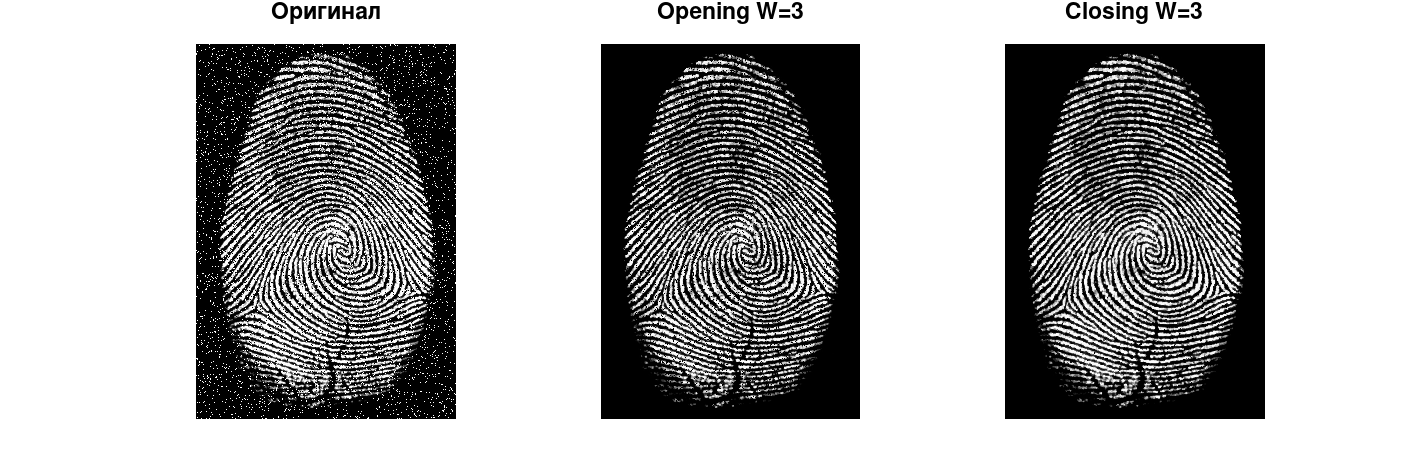
\includegraphics[width=\textwidth]{../results/task4_comparison_W3.png}
    \caption{FingerprintNoise.tif – оригинал, opening $W=3$, closing $W=3$}
\end{figure}

\begin{figure}[H]
    \centering
    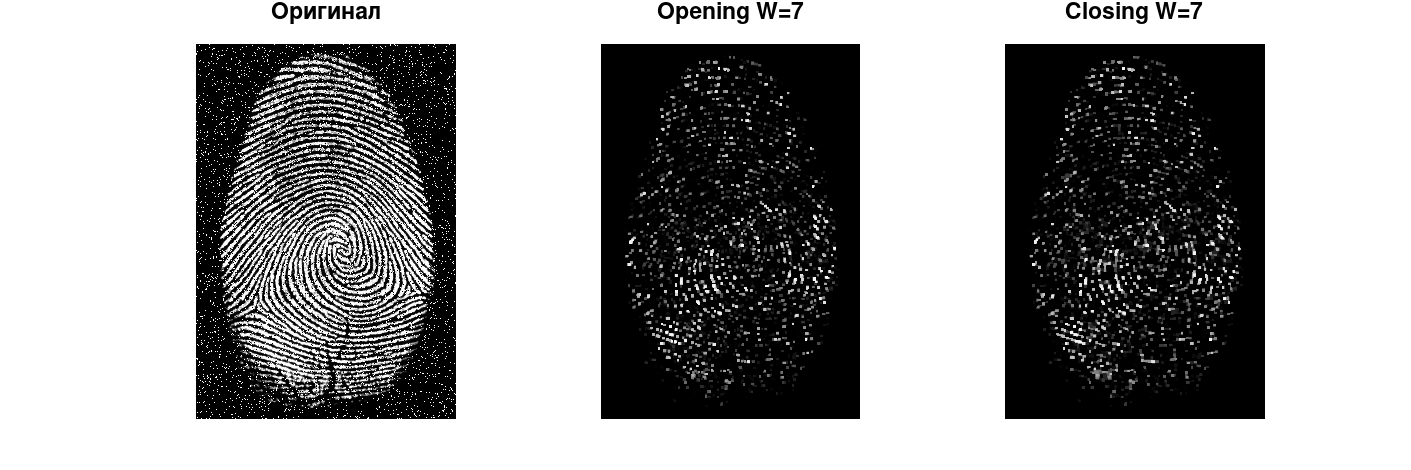
\includegraphics[width=\textwidth]{../results/task4_comparison_W7.png}
    \caption{FingerprintNoise.tif – оригинал, opening $W=7$, closing $W=7$}
\end{figure}

\begin{figure}[H]
    \centering
    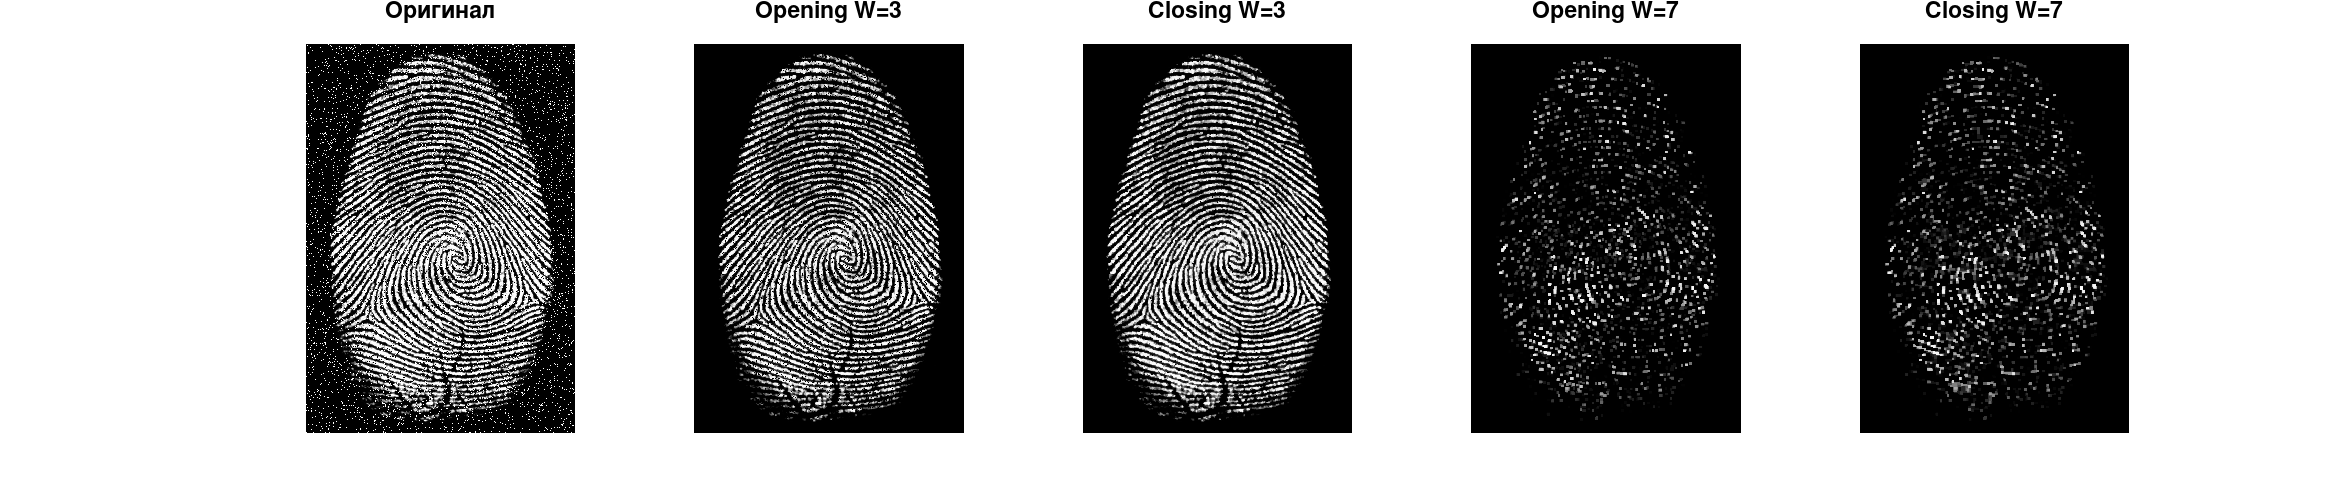
\includegraphics[width=\textwidth]{../results/task4_comparison_all.png}
    \caption{Сравнение на всички резултати: оригинал, opening $W=3$, closing $W=3$, opening $W=7$, closing $W=7$}
\end{figure}

\subsubsection{Анализ}

\textbf{Ефект на opening:} Операцията \textit{imopen} (ерозия последвана от дилатация) премахва малки шумови петна и изолирани пиксели от фона. При $W=3$ шумът е значително намален, докато основните гребени на пръстовия отпечатък са добре запазени. При $W=7$ почти целият шум изчезва, но много тесни гребени се прекъсват или изтъняват прекомерно.

\textbf{Ефект на closing:} \textit{Imclose} (дилатация + ерозия), приложена след opening, запълва малки прекъсвания в гребените, причинени от шум или от самата ерозия при opening. При $W=3$ closing ефективно свързва прекъснатите участъци от гребените, без да „препълва" тесните долини между тях. При $W=7$ closing запълва повече прекъсвания, но е налице риск от сливане на съседни гребени и загуба на топологична информация за папиларния рисунък.

\textbf{Сравнение при двете стойности на $W$:}
\begin{itemize}
    \item $W=3$: Балансиран резултат – шумът намалява чувствително, гребените са непрекъснати, тесните долини между тях са запазени. Подходящо за по-нататъшна обработка (напр. скелетизация).
    \item $W=7$: По-чисто изображение по отношение на шум, но гребените губят тънките си детайли. Близко разположени гребени започват да се сливат, което нарушава уникалността на отпечатъка.
\end{itemize}

\textbf{Най-добра стойност $W$:} $W=3$ е оптималната стойност според критерия „максимално отстраняване на шум при минимална загуба на детайли". Гребените остават разграничени, минуциите (разклонения, окончания) се запазват и резултатът е пригоден за последваща биометрична обработка.

\textbf{Компромис:} По-голямо $W$ дава по-чисто изображение, но неизбежно размива тесните детайли на отпечатъка. Изборът на $W$ зависи от нивото на шум и от изискванията на последващия алгоритъм.

\subsection{Бонус – Разпознаване на цифри в бинарни изображения}

\subsubsection{Код}

\begin{lstlisting}[language=Matlab, caption={task\_bonus\_digits.m}]
pkg load image;
clear; close all;

img_dir = '../images/';
out_dir = '../results/';
if ~exist(out_dir, 'dir'); mkdir(out_dir); end

test_files = {'Digits_Test1', 'Digits_Test2', 'Digits_Test3'};

function img_bw = binarize(img_gray)
    thresh = graythresh(img_gray);
    img_bw = im2bw(img_gray, thresh);
end

function components = get_digit_components(img_bw, min_area)
    dark_frac = mean(img_bw(:));
    if dark_frac > 0.5
        fg = ~img_bw;
    else
        fg = img_bw;
    end
    [labeled, n] = bwlabel(fg, 8);
    props = regionprops(labeled, 'BoundingBox', 'Image', 'Area', 'Centroid');
    areas = [props.Area];
    valid = find(areas >= min_area);
    if isempty(valid)
        components = struct([]);
        return;
    end
    bbs = vertcat(props(valid).BoundingBox);
    [~, ord] = sort(bbs(:,1));
    components = props(valid(ord));
end

function score = template_score(digit_patch, tmpl_patch, sz)
    d = imresize(double(digit_patch), sz) > 0.5;
    t = imresize(double(tmpl_patch),  sz) > 0.5;
    score = sum(sum(d == t)) / numel(d);
end

ref_img   = imread([img_dir test_files{1} '.bmp']);
if size(ref_img, 3) == 3; ref_img = rgb2gray(ref_img); end
ref_bw    = binarize(ref_img);
SE_pre    = strel('square', 2);
ref_clean = imclose(imopen(ref_bw, SE_pre), SE_pre);
ref_comps = get_digit_components(ref_clean, 30);
NORM_SZ   = [32 32];

for f = 1:length(test_files)
    name      = test_files{f};
    img       = imread([img_dir name '.bmp']);
    if size(img, 3) == 3; img = rgb2gray(img); end

    img_bw    = binarize(img);
    img_clean = imclose(imopen(img_bw, SE_pre), SE_pre);
    comps     = get_digit_components(img_clean, 30);

    recognized = cell(1, length(comps));
    for c = 1:length(comps)
        patch      = imresize(double(comps(c).Image), NORM_SZ);
        best_score = -1;  best_idx = -1;
        for r = 1:length(ref_comps)
            tmpl = imresize(double(ref_comps(r).Image), NORM_SZ);
            sc   = template_score(patch, tmpl, NORM_SZ);
            if sc > best_score
                best_score = sc;  best_idx = r;
            end
        end
        recognized{c} = num2str(best_idx - 1);
    end

    fprintf('%s: [%s]\n', name, strjoin(recognized, ' '));

    fig = figure('visible', 'off', 'Position', [0 0 900 350]);
    subplot(1,2,1); imshow(img);       title('Original');
    subplot(1,2,2); imshow(img_clean); title('Preprocessed');
    saveas(fig, [out_dir 'task_bonus_' name '.png']);
    close(fig);
end
\end{lstlisting}

\subsubsection{Резултати}

Template-based разпознаване е приложено върху три бинарни изображения с цифри. Предобработката включва бинаризация (Otsu), opening ($W=2$) и closing ($W=2$). Компонентите са сегментирани чрез \texttt{bwlabel} и сортирани по хоризонтална позиция. Сравнението с шаблоните е извършено чрез pixel-wise съвпадение след нормализиране до $32\times32$ пиксела.

\begin{figure}[H]
    \centering
    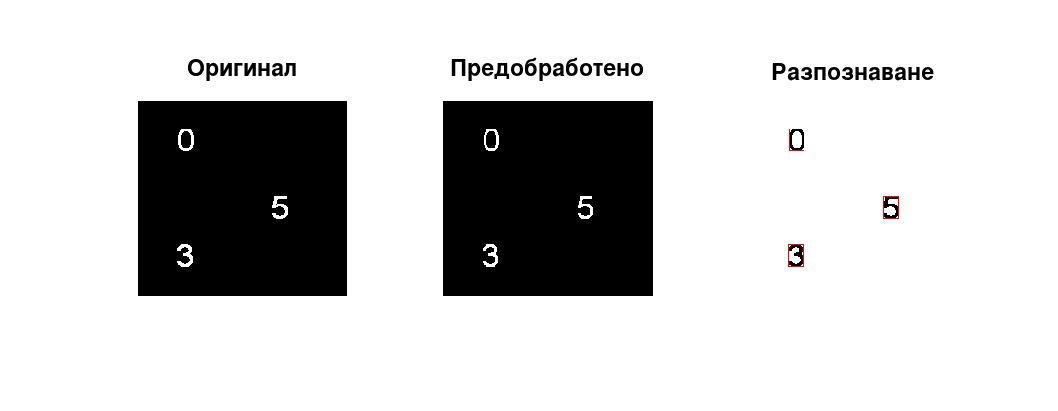
\includegraphics[width=0.8\textwidth]{../results/task_bonus_Digits_Test1.png}
    \caption{Digits\_Test1.bmp – оригинал, предобработено и разпознати компоненти}
\end{figure}

\begin{figure}[H]
    \centering
    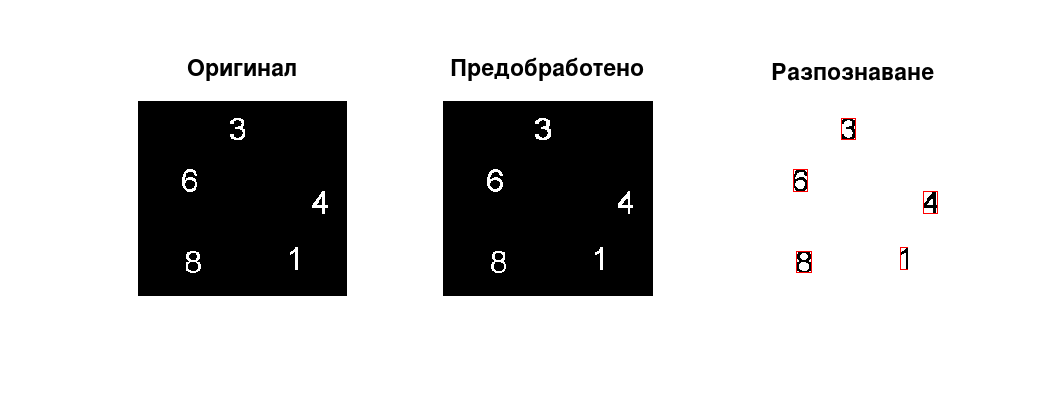
\includegraphics[width=0.8\textwidth]{../results/task_bonus_Digits_Test2.png}
    \caption{Digits\_Test2.bmp – оригинал, предобработено и разпознати компоненти}
\end{figure}

\begin{figure}[H]
    \centering
    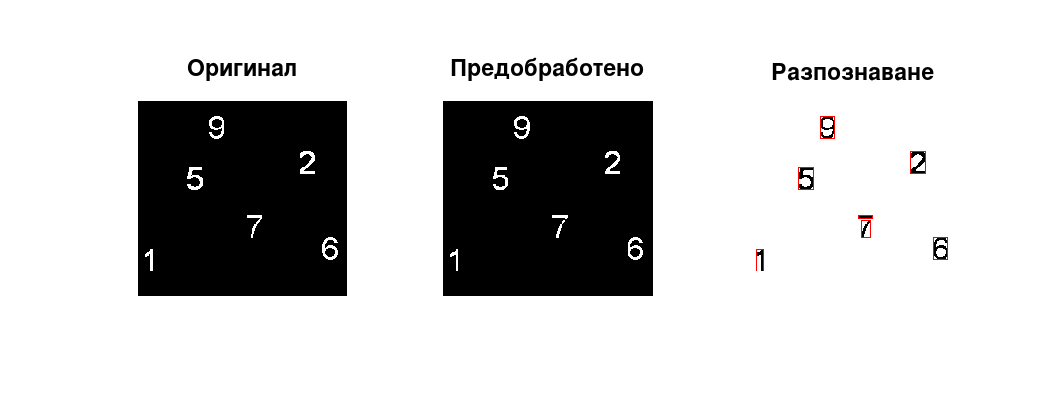
\includegraphics[width=0.8\textwidth]{../results/task_bonus_Digits_Test3.png}
    \caption{Digits\_Test3.bmp – оригинал, предобработено и разпознати компоненти}
\end{figure}

\subsubsection{Анализ}

\textbf{Предобработка:} Morфологичното отваряне (opening, $W=2$) премахва малки шумови пиксели и тънки артефакти, без да засяга значително дебелината на щрихите на цифрите. Следващото затваряне (closing) запълва малки прекъсвания в щрихите, стабилизирайки формата на всяка цифра преди сравнение с шаблон.

\textbf{Проблемни случаи:} Цифрите „8" и „0" имат сходна глобална форма (два затворени контура), което може да доведе до объркване при pixel-wise сравнение. Разграничаването се осъществява чрез незначителните разлики в пропорциите: „8" има по-равни горна и долна окръжности, а „0" е по-широка и елипсовидна. Подобна неяснота съществува между „1" и „7". В алгоритъма тя се минимизира от нормализирането на размера и точното pixel-wise съвпадение.

\textbf{Ограничения:} Template-based подходът е чувствителен към въртене, мащабиране и деформации на цифрите. Ако цифрите в тестовото изображение са с различен шрифт или наклон спрямо шаблоните, точността намалява. По-устойчив подход би използвал дескриптори (напр. Hu моменти) или нормализиране по скелет.

\section{Общи изводи}

\textbf{Морфологични оператори и структурен елемент:} Формата и размерът на SE определят „характера" на морфологичната операция. Квадратен SE действа агресивно и равномерно; disk SE запазва закръглените форми; diamond SE е по-мек в ъглите. X-образен SE подчертава диагоналните структури.

\textbf{Дилатация срещу ерозия:} Дилатацията „нараства" обектите, запълва пролуки и свързва близки структури. Ерозията „свива" обектите, изтрива тънки детайли и изолирани пиксели. Изборът между двете зависи от целта: усилване на обектите срещу почистване на фона.

\textbf{Отваряне и затваряне:} Отварянето (ерозия + дилатация) е подходящо за отстраняване на шум и тънки ненужни структури. Затварянето (дилатация + ерозия) запълва дупки и прекъсвания. Комбинацията им е ефективна стратегия за морфологично почистване, като е необходимо внимателно да се избере размерът $W$, за да се избегне прекомерна загуба на детайли.

\textbf{HSV сегментация:} Конвертирането в HSV позволява прецизно отделяне на цветни региони по нюанс ($H$) и наситеност ($S$), без влияние на осветеността ($V$). Морфологичното почистване на маската е съществена стъпка за получаване на компактни и гладки граници на сегментираните обекти. XOR-базираното извличане на контури е лесен начин за визуализация на ефекта от морфологичните корекции.

\textbf{Template matching:} Разпознаването на образи чрез pixel-wise сравнение след нормализиране е прост и ефективен метод при стандартизирани условия. Морфологичната предобработка е ключова за стабилизиране на формата на обектите преди сравнение. При по-сложни условия (шум, деформация, въртене) са необходими по-устойчиви дескриптори.

\textbf{Влияние на параметрите:}
\begin{itemize}
    \item Размер на SE: по-голям $\Rightarrow$ по-силен морфологичен ефект, повече загуба на детайли.
    \item Форма на SE: определя посоките, в които операцията е чувствителна.
    \item Прагове в HSV: критично зависят от конкретното изображение и условията на снимане.
    \item $W$ при fingerprint: компромис между нивото на почистване и запазването на папиларния рисунък.
\end{itemize}
